\newcommand{\RW}{\italMathId{RW}}
\newcommand{\size}{\italMathId{size}}
\newcommand{\Sizeof}{\italMathId{sizeof}}
%\newcommand{\NULL}{\italMathId{null}}
\newcommand{\LIMIT}{\italMathId{LIMIT}}

\section{\clsm\ Algorithm}
\label{sec:algorithm}

% efficient concurrent operations
We now present \clsm, our algorithm for concurrency support in an LSM-DS.
Section~\ref{Se:Basic} presents our basic approach for providing scalable concurrent \scode{get} and \scode{put} operations; this solution is generic, and can be integrated with many LSM-DS implementations.
In Section~\ref{Se:Snapshots}, we extend the functionality with snapshot scans,
which are implemented in state-of-the-art key-value stores (e.g.,~\cite{leveldb,Hyperdex2012}).
This extension assumes that the in-memory data structure supports ordered iterated access with weak consistency (explained below),
as various in-memory data structures do (e.g.,~\cite{ConcurrentSkipListMap,bronson2010practical,libcds}).
Finally, in Section~\ref{Se:RMW}, we provide general-purpose
non-blocking atomic read-modify-write operations. These are supported in the context of a specific implementation of the
in-memory store as a skip list data structure (or any collection of sorted linked lists).

\clsm\ optimizes in-memory access in the LSM-DS, while ensuring correctness of the entire data store.
Specifically, if the in-memory component's operations ensure
serializability~\cite{Papadimitriou1979}, then the same is guaranteed by the
resulting LSM-DS.

\remove{
\clsm\ is almost entirely non-blocking (lock-free) in that it does not block threads during normal in-memory operation:
If the underlying implementation of the in-memory component is non-blocking, then,
other than inherent blocking of the LSM-DS (when get searches the disk component or put blocks
due to hard size limits of the in-memory components), \clsm\ \emph{never} blocks get operations and
only blocks put operations during short intervals before and after a merge occurs, whilst the global pointers are being updated.
}

\subsection{Put and Get Operations}
\label{Se:Basic}

%In this section we present our support for \scode{put} and \scode{get} operations.
We assume a thread-safe map data structure for the in-memory component,
i.e., its operations can be executed by multiple threads concurrently.
Numerous data structure implementations, (e.g., see \cite{libcds,Herlihy2008,ConcurrencyInWindows2008}), provide this functionality in a non-blocking and atomic manner.
%
In order to differentiate the interface of the internal map data structure from
that of the entire LSM-DS, we refer to the corresponding functions of the in-memory data structure
as \scode{insert} and \scode{find}:
%More precisely, the in-memory data structure supports at least the following two operations:
\begin{description}
\item [\scode{insert(k,v)}] -- inserts the key-value pair $(k,v)$ into the map.
If $k$  exists, the value associated with it is over-written.
%A key is removed by inserting a $\NULL$ value.
\item[\scode{find(k)}] -- returns a value $v$ such that
 the map contains an item $(k,v)$, or $\NULL$ if no such value exists.
\end{description}

The disk component and merge function are implemented in an arbitrary way.

We implement our concurrency support in two hooks, \scode{beforeMerge} and \scode{afterMerge},
which are executed immediately before and immediately after the merge process, respectively.
The merge function returns a pointer to the new disk component, $N_d$, which is passed as a
parameter to \scode{afterMerge}.
The global pointers $P_m$, $P_m^{'}$ to the memory components, and   $P_d$ to
the disk component, are updated during \scode{beforeMerge} and \scode{afterMerge}.

Puts and gets access the in-memory component directly.
Get operations that fail to find the requested key in the current in-memory component search
the previous one (if it exists) and then the disk store.
Recall that  \scode{insert} and \scode{find}
are thread-safe, so we do not need to synchronize \scode{put} and \scode{get}
with respect to each other. However, synchronizing between the update of global
pointers and normal operation is a subtle issue.

We observe that for \scode{get} operations, no blocking synchronization is needed.
This is because the access to each of the pointers is atomic (as it is a
single-word variable).
The order in which components are traversed in search of a key follows
the direction in which the data flows (from $P_m$ to $P_m^{'}$ and from there to
$P_d$) and is the opposite of the order in which the pointers are updated in
\scode{beforeMerge} and \scode{afterMerge}. Therefore, if the pointers
change after \scode{get} has searched the component pointed by $P_m$ or $P_m^{'}$,
then it will search the same data twice, which may be inefficient, but does not violate safety.

\eurosys{I1I2}{
%Following the pointer update,
We use reference counters to avoid freeing a memory component while it is
being read. In addition, we apply an RCU-like mechanism to protect the pointers to memory components 
from being switched while an operation is in the middle of the (short) critical
section in which the pointer is read and its reference counter is increased.
%that are still being accessed by live read operations.
As we only use reference counters per component (and not per row), their overhead
is negligible.
%Our experiments in the next section show that the overhead of such reference counters is negligible.
}

For \scode{put} operations, a little more care is needed to avoid insertion to obsolete in-memory components.
This is because such insertions may be lost in case the merge process has already traversed the
section of the data structure where the data is inserted.
To this end, we use a shared-exclusive lock (sometimes called readers-writer lock~\cite{ConcurrencyInWindows2008}),
 \emph{Lock}, in order to synchronize between \scode{put} operations
and the global pointers' update in \scode{beforeMerge} and \scode{afterMerge}.
(Such a lock does  not block shared lockers  as long as no exclusive locks are requested.)
The lock is acquired in shared mode during the \scode{put} procedure,
and in exclusive mode during \scode{beforeMerge} and \scode{afterMerge}.
In order to avoid starvation of the merge process, the lock implementation should prefer
exclusive locking over shared locking. Such a lock implementation is given, e.g., in~\cite{libcds}.

The basic algorithm is implemented by the four procedures in \algref{basicAlg}.
%\Idit{Added below but not sure if it belongs here or in Section 2}.
%For persistence, put operations also need to also write to the log (omitted from the pseudo-code). As in most systems~\cite{XXX}, this is done asynchronously and is therefore does not induce blocking.

\begin{algorithm} [th!]
\small
\caption{\small  Basic \clsm\ algorithm.}
\label{alg:client}
%
\begin{algorithmic}[1]
\makeatletter\setcounter{ALG@line}{0}\makeatother
%
\Procedure{put}{Key $k$, Value $v$}
     \State \emph{Lock}.lockSharedMode() \label{beginPut1}
     \State $P_{m}$.insert($k,t$)
     \State \emph{Lock}.unlock()
\EndProcedure
%
\vspace{3pt}
%
\Procedure{get}{Key $k$}
    \State $v \gets$ find $k$ in $P_{m}$, $P'_{m}$, or $P_{d}$, in this order
    \State return $v$
\EndProcedure
%
\vspace{3pt}
%
\Procedure{beforeMerge}{}
   \State \emph{Lock}.lockExclusiveMode()
   \State $P_{m}^{'} \gets P_{m}$
   \State $P_{m} \gets$ new in-memory component
   \State \emph{Lock}.unlock()
\EndProcedure
%
\vspace{3pt}
%
\Procedure{afterMerge}{DiskComp $N_d$}
   \State \emph{Lock}.lockExclusiveMode()
   \State $P_{d} \gets N_d$
   \State $P_{m}^{'} \gets \NULL$
   \State \emph{Lock}.unlock()
\EndProcedure
\end{algorithmic}
\label{Al:basicAlg}
\end{algorithm}

\subsection{Snapshot Scans}
\label{Se:Snapshots}


We implement serializable snapshot scans using the common approach of multi-versioning: each key-value pair is  stored in the map together with a unique, monotonically increasing, timestamp. That is,
the elements stored in the underlying map are now key-timestamp-value triples.
The timestamps are internal, and are not exposed to the LSM-DS's application.

Here, we assume the underlying map is sorted in lexicographical order of the key-timestamp pair. Thus, \scode{find} operations can return the value associated with the highest timestamp for a given key.
We further assume that the underlying map provides iterators with the
so-called \emph{weak consistency} property, which guarantees that if an element is included in the data structure for the entire duration of a complete snapshot  scan, this element is returned by the scan.
Several map data structures and data stores support such sorted access and iterators with weak consistency (see~\cite{ConcurrentSkipListMap,bronson2010practical}).

To support multi-versioning, a \scode{put} operation acquires a timestamp before
inserting a value into the in-memory component.
This is done by atomically incrementing and reading a global counter, \emph{timeCounter};
there are non-blocking implementations of such counters (e.g., see~\cite{ConcurrencyInWindows2008}).
A \scode{get} operation now returns the highest timestamped value for the given key.

Our support for snapshots and full scans thereof is explained in Section~\ref{se:snapshot-mechanism}.
We discuss other snapshot-based operations (like range queries) in Section~\ref{se:range}.

\subsubsection{Snapshot Management Mechanism}
\label{se:snapshot-mechanism}

A snapshot is associated with a timestamp, and contains, for each key, the
latest value updated up to this timestamp.
Thus, although a snapshot scan spans multiple operations, it
reflects the state of the data at a unique point in time.

The \scode{getSnap} operation returns a snapshot handle $s$, over which
subsequent operations may iterate.
In \clsm, a snapshot handle is simply a timestamp $ts$.
A scan iterates over all live components (one or two
memory components and the disk component) and filters out items that do not
belong to the snapshot:
for each key $k$, the \scode{next} operation filters out items that have higher
timestamps than the snapshot time, or are older than the latest timestamp (of key $k$) that does not exceed the snapshot time.
%Note that since $P_m$ always holds the latest inserted values, and $P_m^{'}$
%holds values no older than those in $P_d$, \scode{next} may return as soon as it finds a value older than the requested snapshot
%either in $P_m$ or in $P_m^{'}$.
When there are no more items in the snapshot, \scode{next} returns $\bot$.

Our snapshot management algorithm appears in \algref{snapAlg}.
Determining the timestamp of a snapshot is a bit subtle.
In the absence of concurrent operations, one could simply read the current value
of the global counter.
%
However, in the presence of concurrency, this approach may lead to
inconsistent scans, as illustrated in Figure~\ref{fig:snap-ts}. In this
example, \scode{next} operations executed in snapshot $s_2$, which reads
$98$ from \emph{timeCounter}, filter out a key written with timestamp
$99$, while \scode{next} operations executed in snapshot $s_1$, which reads timestamp
$99$, read this key, but miss a key written with timestamp $98$. The latter is missed because the
\scode{put} operation writing it updates \emph{timeCounter} before the
\scode{getSnap} operation, and inserts the key into the underlying map after the
\scode{next} operation is completed.
This violates serializability as there is no way to serialize the two scans.

\begin{figure}[t]
   		{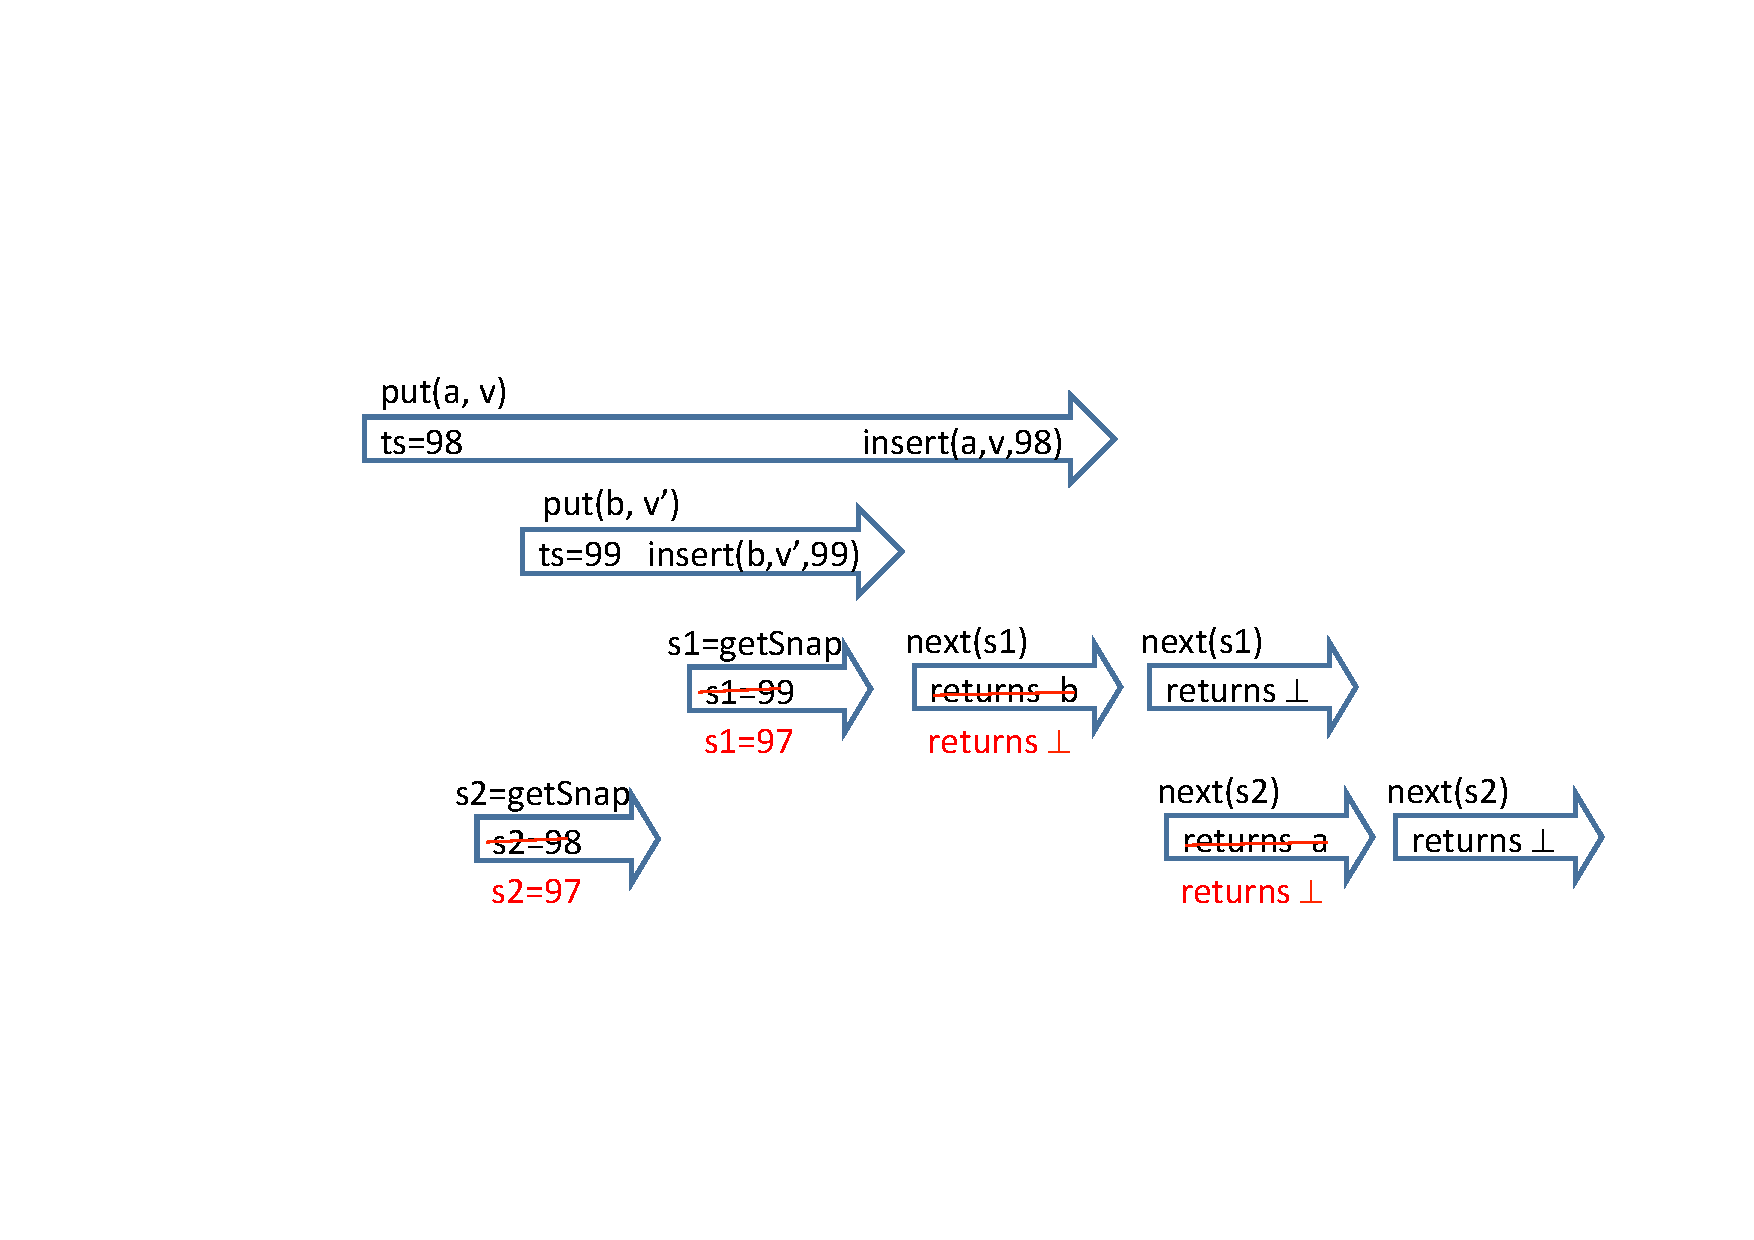
\includegraphics[width=\columnwidth, clip, trim=150 150 50
 		170]{Figures/scanExample}}

		\caption{Snapshots $s_1$ and $s_2$ cannot use the current
		values of \emph{timeCounter}, $99$ and $98$ respectively, since a \scode{next}
		operation pertaining to snapshot $s_1$ may miss the concurrently written key
		$a$ with timestamp $98$, while a \scode{next}
		operation pertaining to snapshot $s_2$ filters out the key $b$ with timestamp $99$.
		The snapshot time should instead be $97$, which excludes the concurrently
		inserted keys.}
\label{fig:snap-ts}
\end{figure}

We remedy this problem by tracking timestamps that were obtained but
possibly not yet written. These are kept in a set data structure, \emph{Active}, which can
be implemented in a non-blocking manner. The \scode{getSnap}
operation chooses a timestamp that is earlier than all active ones.
In the above example, since both $98$ and $99$ are active at the time
$s_1$ and $s_2$ are invoked, they choose $97$ as their snapshot time.


Note that a race can be introduced between obtaining a timestamp and inserting
it into \emph{Active} as depicted in Figure~\ref{fig:race}. In this example, a
\scode{put} operation reads timestamp $98$ from \emph{timeCounter}, and before
it updates the \emph{Active} set to include it, a
\scode{getSnap} operation reads timestamp $98$ from \emph{timeCounter} and finds
the \emph{Active} set empty. The snapshot timestamp is therefore set to $98$.
The value later written by the \scode{put} operation is not filtered out by
the scan, which may lead to inconsistencies, as in the previous example.
%
To overcome this race, the \scode{put} operation verifies that its chosen timestamp exceeds the latest snapshot's timestamp
(tracked in the \emph{snapTime} variable), and re-starts if it does not,
\eurosys{}{while \scode{getSnap} waits until all active \scode{put} operations
have timestamps greater than
\emph{snapTime}.%~\ref{code:snap:blocking}.
}

\begin{figure}[t]
\center
		{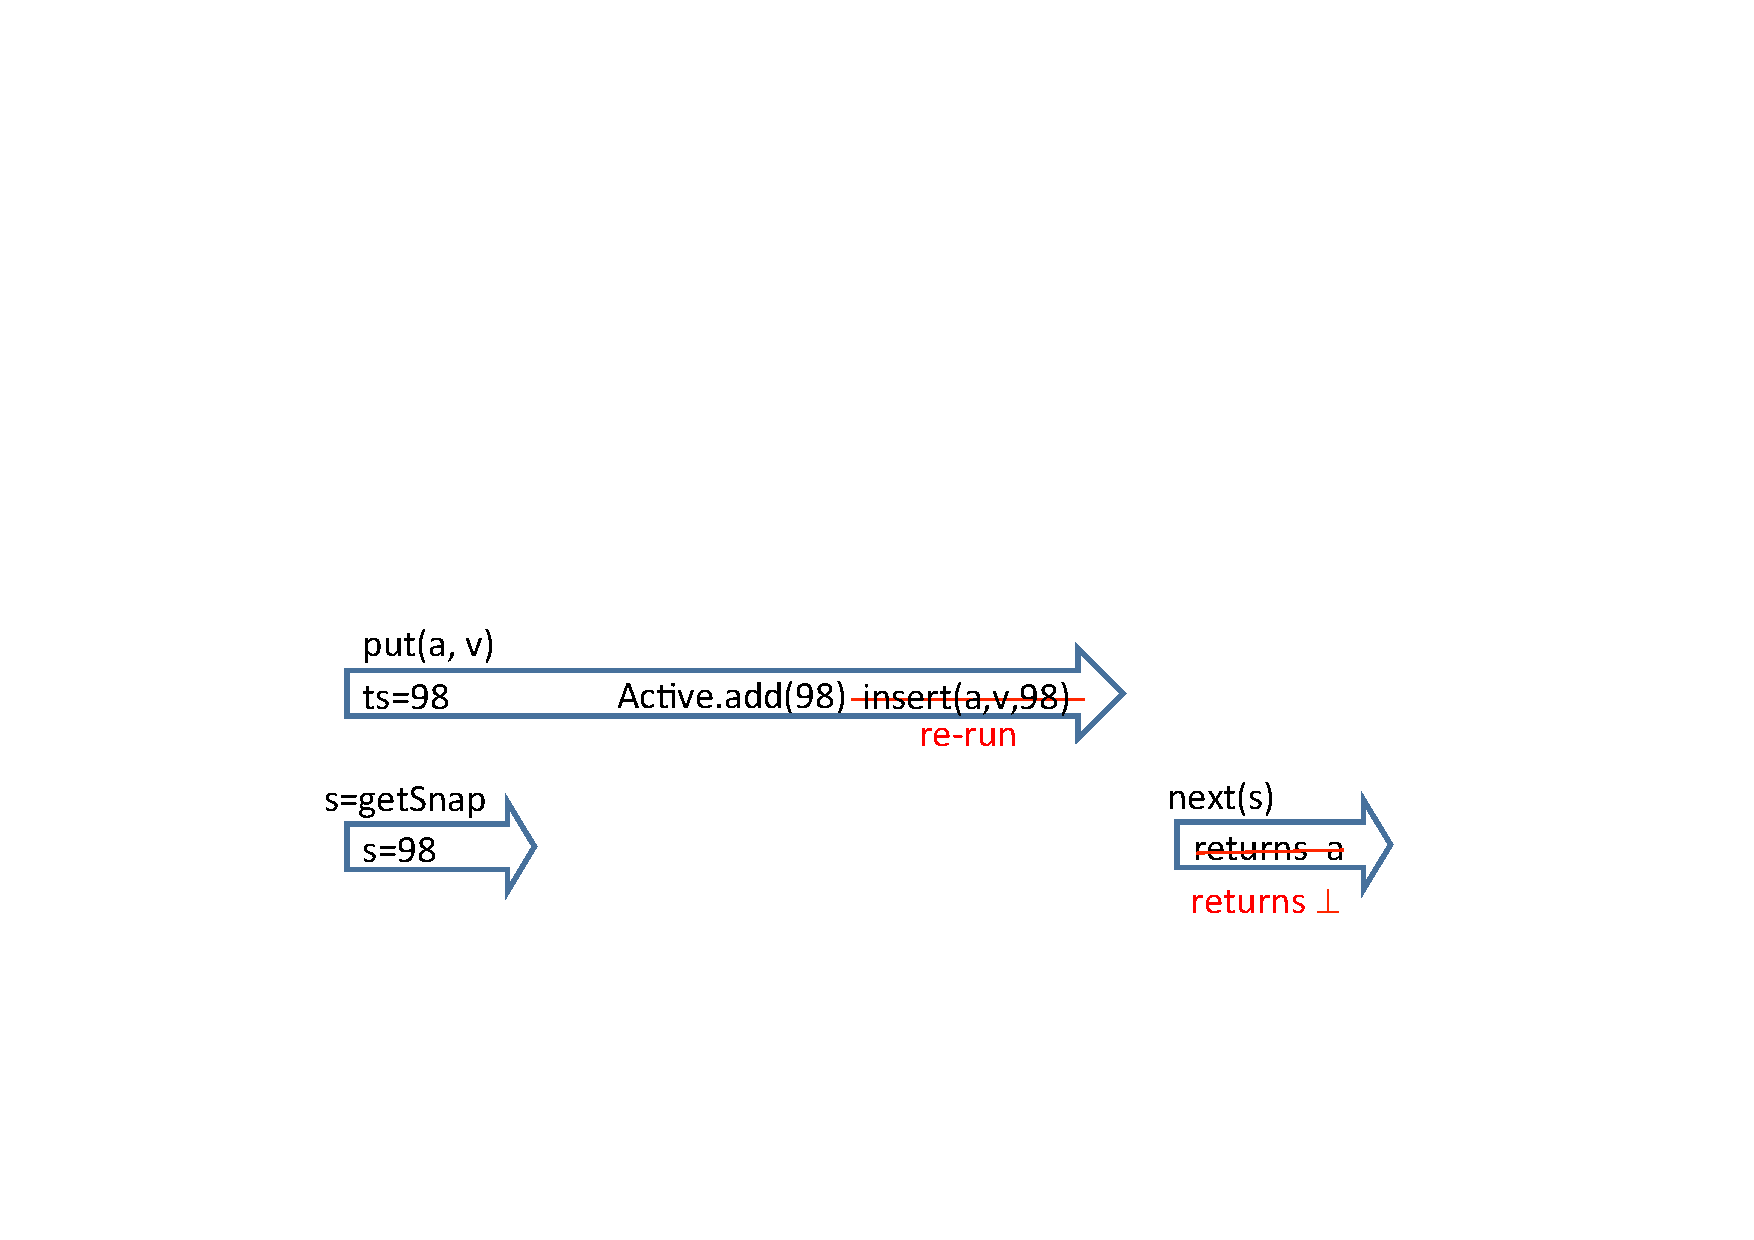
\includegraphics[width=\columnwidth, clip, trim=100 150 100
		300]{Figures/example3}}

		\caption{The put operation cannot use the value $98$ since a
		snapshot operation already assumes there are no active put operations
		before timestamp $99$. Using the timestamp $98$ may lead to the problem
		depicted in Figure~\ref{fig:snap-ts}. The put operation should instead
		acquire a new timestamp.}
  \label{fig:race}
\end{figure}

We note that our scan is serializable but not linearizable~\cite{Herlihy:1990}, in the sense that it can read a consistent state ``in the past''.
That is, it may miss some recent updates,
(including ones written by the thread executing the scan). To preserve
%the \emph{per-thread order}
linearizability, the \scode{getSnap} operation could be modified to wait until it is able
to acquire a \emph{snapTime} value greater than the  \emph{timeCounter}
value at the time the operation started. 
\eurosys{}{This can be done by omitting
lines~\ref{code:active:ts}-\ref{code:snap:ts} in
\algref{snapAlg}. }
%However, in cases where a thread is not
%required to scan its own updates this blocking implementation is not necessary.

Since puts are implemented as insertions with a new timestamp, the key-value store potentially holds many versions for a given key.
Following standard practice in LSM-DS,
old versions are not removed from the memory component, i.e., they exist at least until the component is discarded following its merge into disk.
Obsolete versions are removed during a merge once they are no longer needed for any snapshot.
In other words, for every key and every snapshot, the latest version of the key
that does not exceed the snapshot's timestamp is kept. % in some component.
%We assume an API for installing and removing snapshots which allows reclamation
%of associated values by the merge.

To consolidate with the merge operation, \scode{getSnap} installs the snapshot
handle in a  list  that captures all active snapshots.
Ensuing merge operations query the list to identify the maximal
timestamp before which versions can be removed. To avoid a race between installing a snapshot
handle and it being observed by a merge, the data structure is accessed while
holding the lock. The \scode{getSnap} operation acquires the lock in
shared mode while updating the list, and \scode{beforeMerge} queries the list while holding the
lock in exclusive mode. The timestamp returned by
\scode{beforeMerge} is then used by the merge operation to determine which
elements can be discarded. 
\eurosys{I3}{
%We assume there is a function that removes snapshots by
%removing their handles from the list, either per a user's request, or based on
% TTL.
As in levelDB, we assume handles of unused snapshots are removed
from the list either by the application (through an API call), or based on TTL;
failing to do so may reduce the amount of available memory for useful data.}
%an API for removing the snapshot handle
%from the list when the snapshot is discarded (omitted from the pseudocode).

\begin{algorithm} [t]
\small
\caption{\small  \clsm\ snapshot algorithm.}
\label{alg:snap}
%
\begin{algorithmic}[1]
\makeatletter\setcounter{ALG@line}{0}\makeatother
%
\Procedure{put}{Key $k$, Value $v$}
    \State \emph{Lock}.lockSharedMode()
		\State $ts \gets$ getTS()
    \State $P_{m}$.insert($k,ts,v$)
    \State \emph{Active}.remove($ts$)
    \State \emph{Lock}.unlock()
\EndProcedure
%
\vspace{3pt}
%
% \Procedure{get}{Key $k$}
% %	  \If {$s=\NULL$ } $s \gets \infty$ \EndIf
%     \State find $v$ s.t.\ $(k,ts,v)$ has
%     	highest $ts$ in $P_{m}$, $P'_{m}$, or $P_{d}$
%     \State return $v$
% \EndProcedure
% %
% \vspace{3pt}
% %
% \Procedure{next}{Snapshot $s$}
% %	\Repeat
%     \State $k \gets$ smallest key greater than \emph{current} in $P_{m}$,
%     $P'_{m}$, and $P_{d}$  %in $\{K\}$
%     \State \emph{current} $\gets k$
%     \State find $v$ s.t.\ $(k,ts,v)$ has
%     	highest $ts \leq$ $s$ in $P_{m}$, $P'_{m}$, or $P_{d}$
% %    \Until {$v$ is not marked as deleted}
%     \If {$v$ is marked as deleted} restart \EndIf
%     \State return $\langle k, v \rangle$
% \EndProcedure%
% \vspace{3pt}
%
\Procedure{getSnap}{}
    \State \emph{Lock}.lockSharedMode()
    \State $ts \gets$ \emph{timeCounter}.get()
    \State $ts_a \gets$ \emph{Active}.findMin() \label{code:active:ts}
    \If {$ts_a \not= \NULL$} $ts \gets ts_a - 1$ \EndIf \label{code:snap:ts}
    \State atomically assign $\max(ts, snapTime)$ to \emph{snapTime}  \label{LineSnapTime}
    \While{\emph{Active}.findMin() $<$ \emph{snapTime}} nop
    \label{code:snap:blocking} \EndWhile \State $ts_b \gets snapTime$
    \State install $ts_b$ in the active snapshot list
    \State \emph{Lock}.unlock()
    \State return $ts_b$
\EndProcedure
%
\vspace{3pt}
%
\Procedure{getTS}{}
		\While{\emph{true}}
			\State $ts \gets$ \emph{timeCounter}.incAndGet()
			\State \emph{Active}.add($ts$)
			\If {$ts \leq$ \emph{snapTime} } 	\emph{Active}.remove($ts$) \Else \emph{
			break} \EndIf
		\EndWhile
		\State return $ts$
\EndProcedure
\vspace{3pt}
%
\Procedure{beforeMerge}{}
   \State \emph{Lock}.lockExclusiveMode()
   \State $P_{m}^{'} \gets P_{m}$
   \State $P_{m} \gets$ new in-memory component
   \State $ts \gets$ find minimal active snapshot timestamp
   \State \emph{Lock}.unlock()
   \State return $ts$
\EndProcedure
%

\end{algorithmic}
\label{Al:snapAlg}
\end{algorithm}

\remove{
Our snapshot management algorithm appears in \algref{snapAlg}.
The \scode{put}
and \scode{getSnap} procedures select timestamps as explained above.
The  \scode{get} operation now returns the highsest timestamped value for the given key.
% The \scode{next} operation takes a snapshot as a parameter, and returns, for every key found by the components' iterators,
% the value associated with the highest timestamp smaller than the snapshot time.
Note that since $P_m$ always holds the latest inserted values, and $P_m^{'}$
holds values no older than those in $P_d$, \scode{get} may return as soon as it finds a value older than the requested snapshot
either in $P_m$ or in $P_m^{'}$.
}

Because more than one  \scode{getSnap} operation can be executed concurrently,
we have to update  \emph{snapTime}  with care, to ensure that it does not move backward in time.
We therefore atomically advance \emph{snapTime} to $ts$ 
(e.g., using a CAS\footnote{\emph{Compare and Swap} operation~\cite{Herlihy2008}.}) in line \ref{LineSnapTime}.
%
The rollback loop in \scode{getTS} may cause the starvation of a \scode{put}
operation. We note, however, that each repeated attempt to acquire a timestamp
implies the progress of some other \scode{put} and \scode{getSnap} operations, as expected in non-blocking
implementations.

\subsubsection{Partial Scans and Snapshot Reads}
\label{se:range}

A full snapshot scan traverses
all keys starting with the lowest and ending with the highest one. More common
are partial scans, (e.g., range queries),
in which the application only traverses a small consecutive range of the keys,
or even simple reads of a single key from the snapshot.
Given our snapshot management mechanism, it is straightforward to support these by using
a \eurosys{I5}{find function to locate the first entry to be retrieved (like
finding a key in a \scode{get} operation)}.

\subsection{Atomic Read-Modify-Write}
\label{Se:RMW}

We now introduce a general read-modify-write operation, \scode{RMW(k,f)}, which atomically applies an
arbitrary function $f$ to the current value $v$ associated with key $k$ and stores $f(v)$
in its place.
Such operations are  useful for many applications, ranging from simple vector clock update and validation to implementing full-scale transactions.

%Many state-of-the-art data store implementations  do not provide such general atomic read-modify-write operations. Nevertheless, such operations are extremely useful for many applications, ranging from simple vector clock update and validation to implementing full-scale transactions.

Our solution is efficient and avoids blocking. It is given in
the context of a specific implementation of the in-memory data store as a linked
list or any collection thereof, e.g., a skip-list. Each entry in the linked list
contains  a key-timestamp-value tuple, and the linked list is sorted in
lexicographical order. In a non-blocking implementation of such a data
structure, \scode{put} updates the \emph{next} pointer of the
predecessor of the inserted node using a CAS operation~\cite{Herlihy2008}.

The pseudo-code for read-modify-write on an in-memory linked-list appears in
\algref{RMWAlg}.
The  idea is to use optimistic concurrency control -- having read $v$ as the latest
value of key $k$, our attempt to insert $f(v)$ fails (and restarts) in case a new value has been inserted for $k$ after $v$.
This situation is called a \emph{conflict},
and it means that some concurrent operation has interfered between our read step in line~\ref{LineReadTuple} and our update step in  line~\ref{CASLine}.

\begin{algorithm} [t]
\small
\caption{\small RMW algorithm for linked list memory component.}
\label{alg:RMW}
%
\begin{algorithmic}[1]
\makeatletter\setcounter{ALG@line}{0}\makeatother
%
\Procedure{RMW}{Key $k$, Function $f$}
    \State \emph{Lock}.lockSharedMode()
		\Repeat
	    \State find $(k,ts,v)$ with highest $ts$ in  $P_{m}$, $P'_{m}$, or $P_{d}$ \label{LineReadTuple}
  	  \State \emph{prev} $\gets$ $P_{m}$ node with $\max (k',ts') \leq (k,\infty)$ \label{LineSetPrev}
      \If {\emph{prev.key} $= k$ and \emph{prev.time} $> ts$} continue  \label{conflict1Line}   \EndIf \Comment{conflict}
  	  \State \emph{succ} $\gets$ \emph{prev.next} \label{LineSetNext}
  	  \If {\emph{succ.key} $= k$} continue  \label{conflict2Line}  \Comment{conflict} \EndIf
	  	\State $ts_n \gets$ getTS() \label{newTS}
    	\State create \emph{newNode} with $(k,ts_n,f(v))$
    	\State \emph{newNode.next} $\gets$ \emph{succ}
	    \State \emph{ok} $\gets$ CAS(\emph{prev.next, succ, newNode}) \label{CASLine}
      \If { $\neg$\emph{ok} } \emph{Active}.remove($ts_n$) \Comment{conflict}
      \EndIf
    \Until { \emph{ok} }	
    \State \emph{Active}.remove($ts_n$)
    \State \emph{Lock}.unlock()
\EndProcedure
%
\end{algorithmic}
\label{Al:RMWAlg}
\end{algorithm}

The challenge is to detect conflicts efficiently.
Here, we take advantage of the fact that all updates occur in RAM, ensuring that all conflicts will be manifested in the in-memory component.
We further exploit the linked list structure of this component.
In line~\ref{LineSetPrev}, we locate, and store in \emph{prev}, the insertion point for the new node.
%
If \emph{prev} is a node holding key $k$ and a timestamp higher than $ts$,
then it means that another thread has inserted a new node for $k$ between lines~\ref{LineReadTuple} and \ref{LineSetPrev} ---
this conflict is detected in line~\ref{conflict1Line}.
%
In line~\ref{conflict2Line}, we detect a conflict that occurs when
another thread inserts a new node for $k$ between lines~\ref{LineSetPrev} and
\ref{LineSetNext} --- this conflict is observed when \emph{succ} is a node
holding key $k$.
%
If the conflict occurs after line~\ref{LineSetNext}, it is detected by failure of the CAS in line~\ref{CASLine}.

%In case $k$ was already in the in-memory list, \emph{prev} is a node holding key $k$, and otherwise, it holds a smaller key.
%A conflict is reflected by a change to the successor of \emph{prev}.
%If it changes before we read it into \emph{succ} in line~\ref{LineSetNext}, we detect the conflict in line~\ref{conflictLine}.
%If the conflict occurs after line~\ref{LineSetNext}, the conflict is detected by failure of the CAS in line~\ref{CASLine}.


\remove{
For example, consider a \scode{RMW} operation on key $15$, and assume that this key is found in
the disk component.
When the operation begins, \emph{prev} is set to some node $n$ holding the largest key smaller than $15$.
Assume now that a concurrent \scode{put} operation inserts a new value for key $15$. This value is
also inserted after $n$.
If  \scode{put}  changes \emph{n.next}  before line~\ref{LineSetNext}, then
the conflict is detected in line~\ref{conflictLine}. If it changes
after the \scode{RMW} operation executes line~\ref{LineSetNext} and before it executes line~\ref{CASLine},
then the CAS fails, and again, the operation restarts.
Otherwise, the \scode{put} operation is ordered after the \scode{RMW}, and there is no conflict.
}

When the data store consists of multiple linked lists, as
\emph{libcds}'s lock-free skip-list does~\cite{libcds}, items are inserted to
the lists one at a time, from the bottom up~\cite{Herlihy2008}.
Only the bottom  list is required for correctness, while the others ensure the
logarithmic search complexity. Our implementation thus
% , like \emph{libcds}'s lock-free skip-list~\cite{libcds},
first inserts the new item
to the bottom list atomically using \algref{RMWAlg}. It then adds the item to each higher list using a CAS as
in line~\ref{CASLine}, but with no need for a new timestamp~\ref{newTS} or
conflict detection as in lines~\ref{conflict1Line} and~\ref{conflict2Line}.

We note that the lock-free skip-list \cite{libcds}
 (which is based on the skip-list algorithm in~\cite{Herlihy2008})
satisfies the requirements specified in Section~\ref{Se:Snapshots} ---
%Although, in the general case, this data structure does not  guarantee weak
% consistency, in our case it does ensure this property.
%In this data structure,
weak consistency is guaranteed as long as items are not
removed from the skip-list, as is the case in \clsm.
% --- and in our algorithm, items are never removed from the skip-list as long as it is being used.
%(Items are removed and freed only when the entire skip-list is freed).




